\begin{figure}
\centering
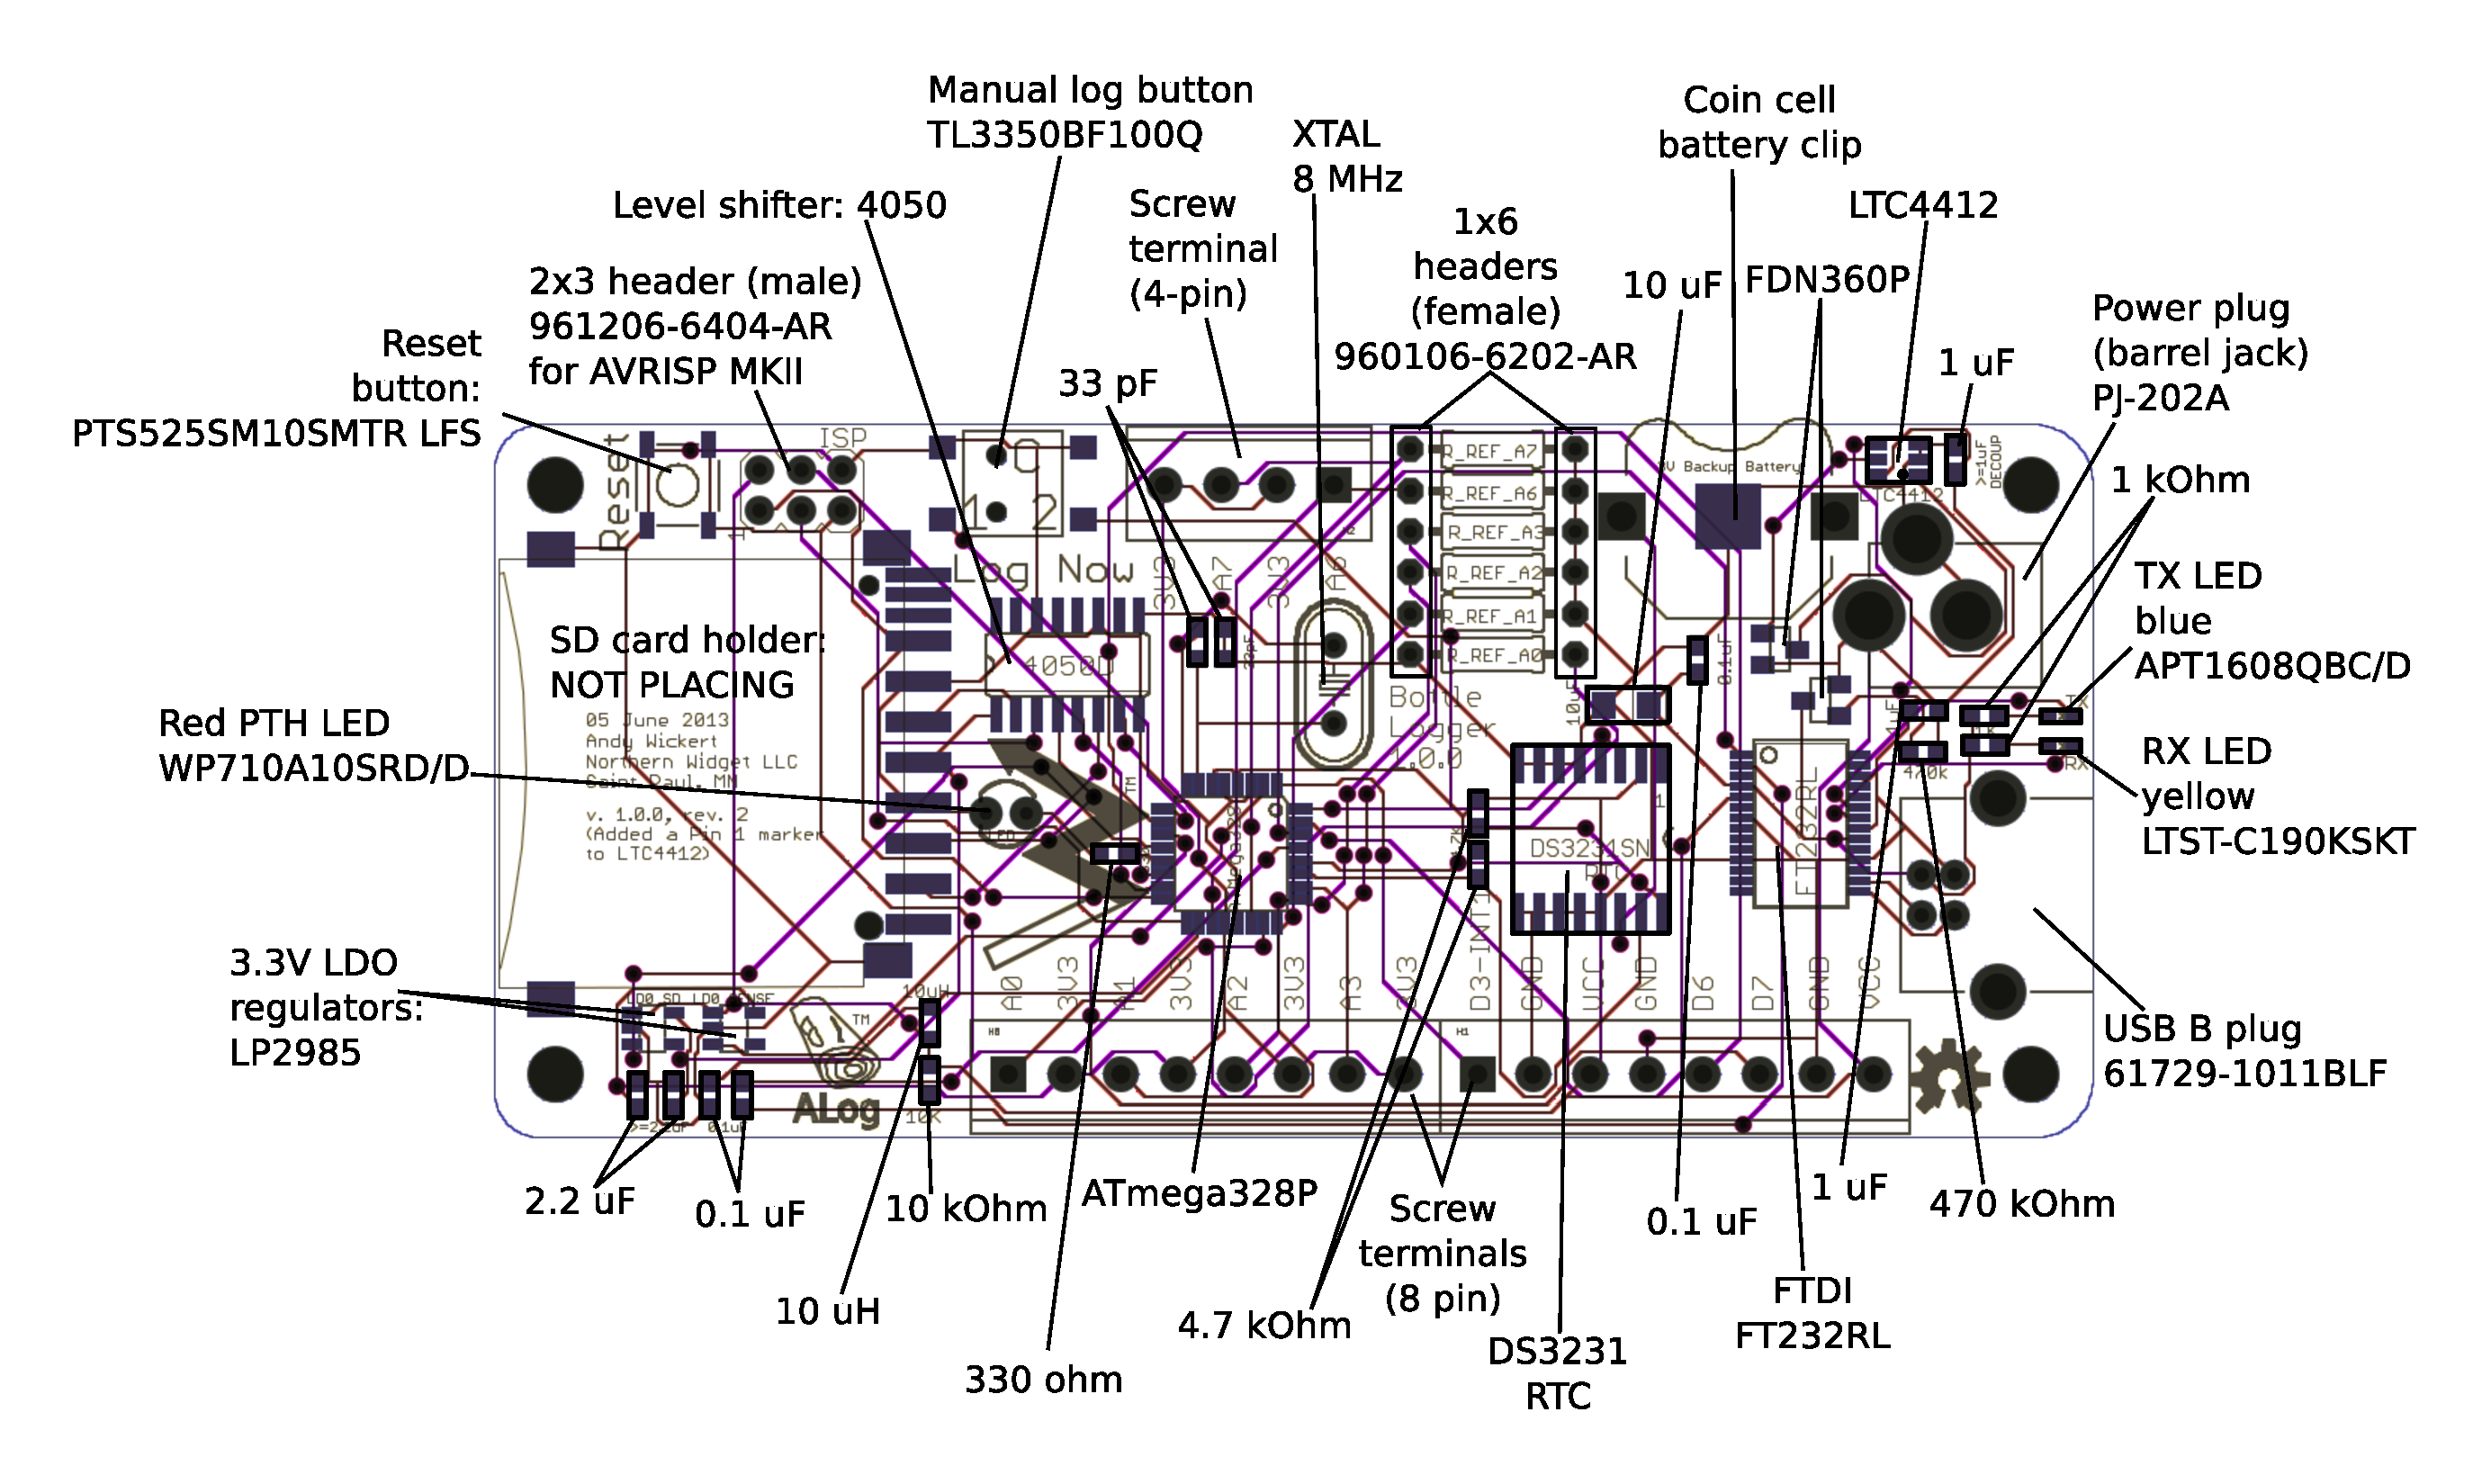
\includegraphics[height=10cm]{graphics/ALog_drawing}
\caption{Arduino-based low-power field environmental data logging platform: hardware schematics and circuit board layouts\label{fig:BottleLog}\cite{ALog-BottleLogger}}
\end{figure}

\section{Background}
Data sampling is a well know method to help scientists understand nature's behavior. Back in the days, scientists sampled data in real time in the field by writing measurements down to log book. With time automatic measurement equipment was developed which made it possible for scientists to leave the field and come back later to collect the data in order to process. Nowadays, with wireless communication technology the automatic measurement equipments allows scientist to access data in real time without going to the field.\\
Similar equipment that fulfills the requirements of being light-weight and affordable with long-range transmit capabilities is unavailable today. The available equipment which is capable of long range communications through GSM network can be seen in figure \ref{fig:a} and \ref{fig:b} and costs around \$ 3,000. A cheaper equipment as shown in figure \ref{fig:c} and  \ref{fig:d} costs around \$ 500 has the disadvantage of limited wireless range only up to 300 meters.

\begin{figure}[H]
  \centering
  \subfloat[\$3500 \label{fig:a}\cite{WeatherShop2014}]
  {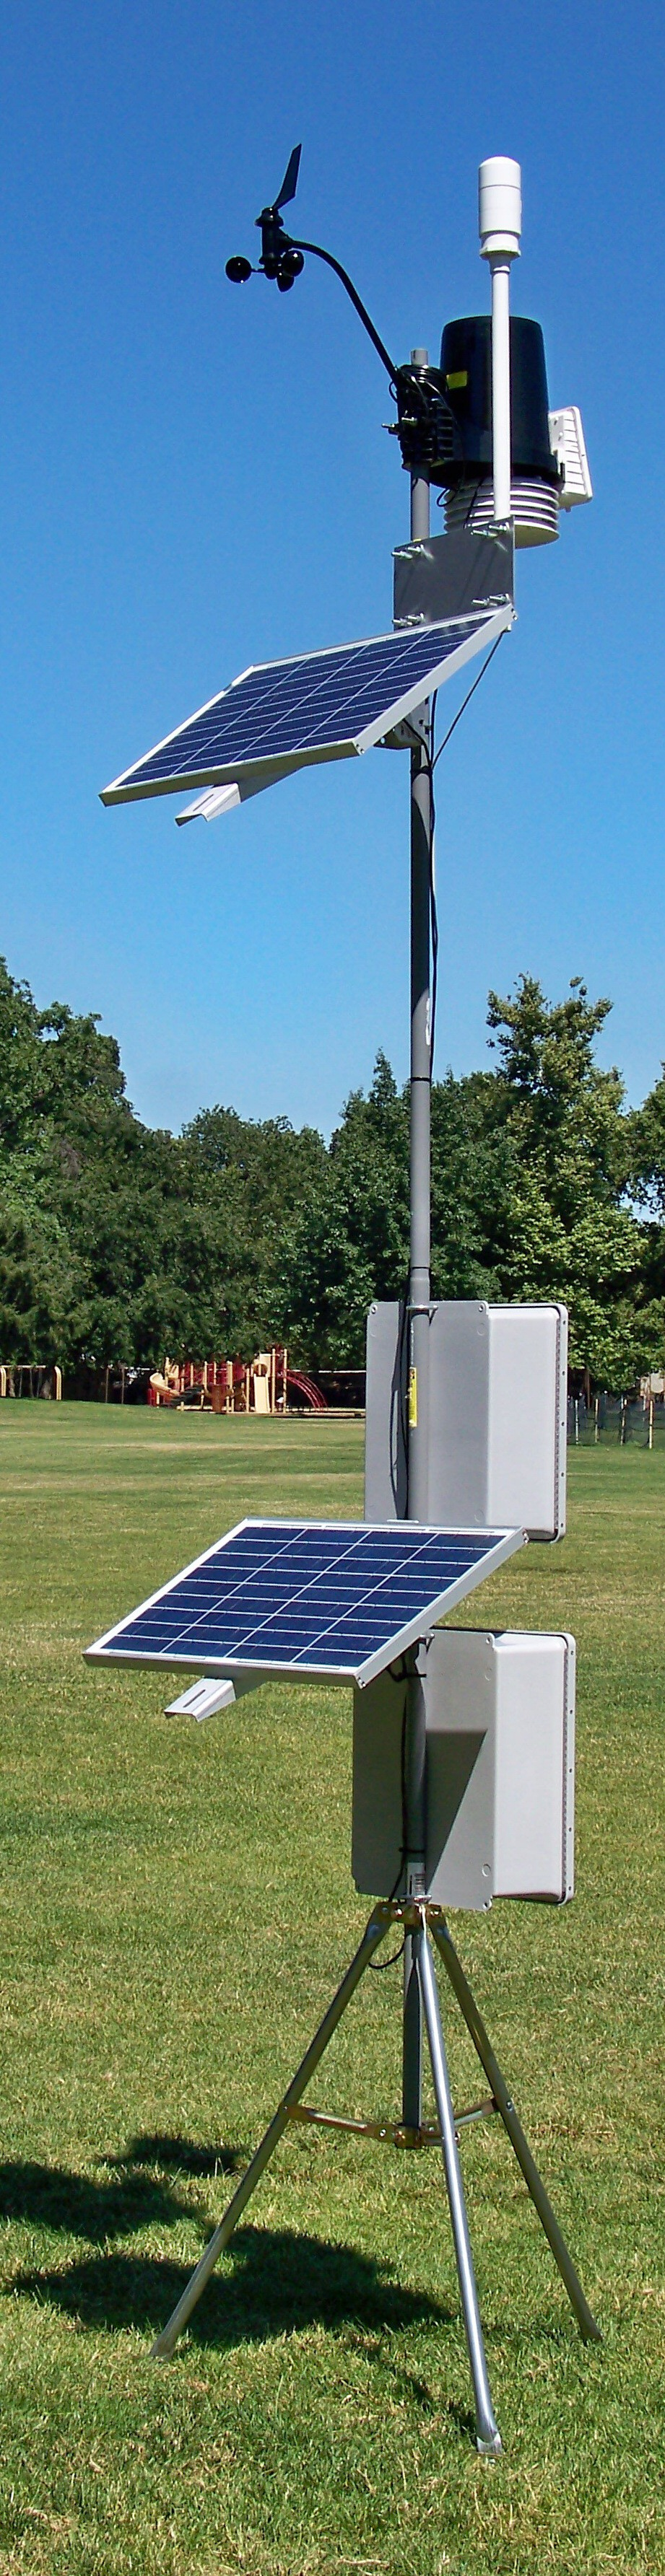
\includegraphics[height=6.5cm]{graphics/cellular_weather_station}}\quad
  \subfloat[\$2800 \label{fig:b}\cite{TexasWeatherInstruments2014}]
  {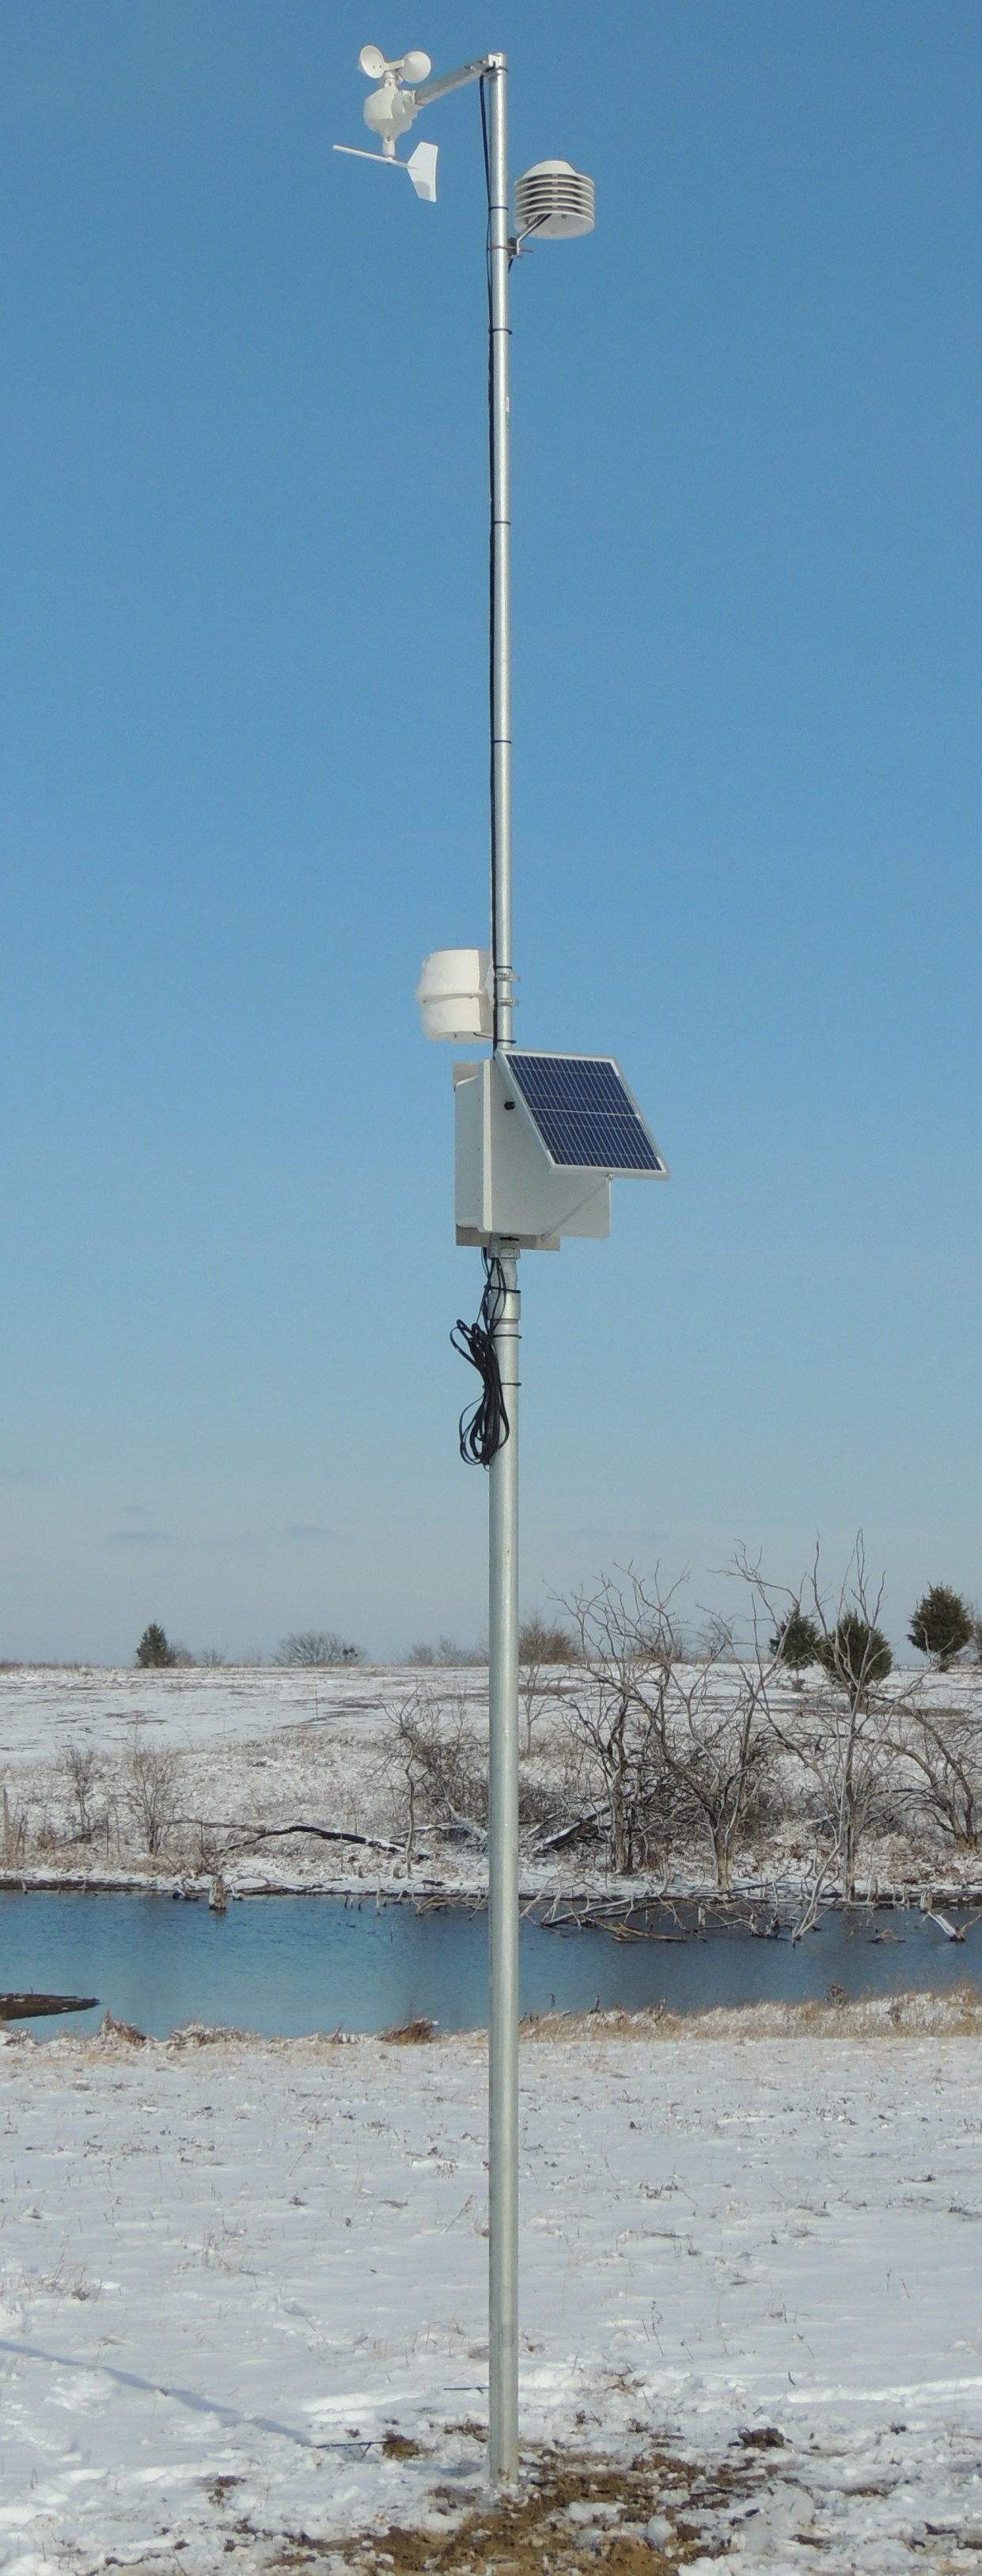
\includegraphics[height=6.5cm]{graphics/RWS-Snow}}\quad
  \subfloat[\$658 \label{fig:c}\cite{Scientific2014}]
  {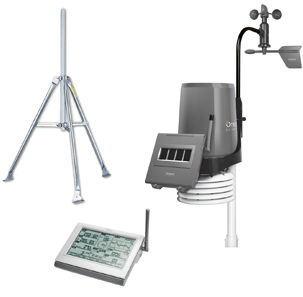
\includegraphics[height=4cm]{graphics/Oregon_Scientific_Pro_weather_system}}\quad
  \subfloat[\$595 \label{fig:d}\cite{Davis2014}]
  {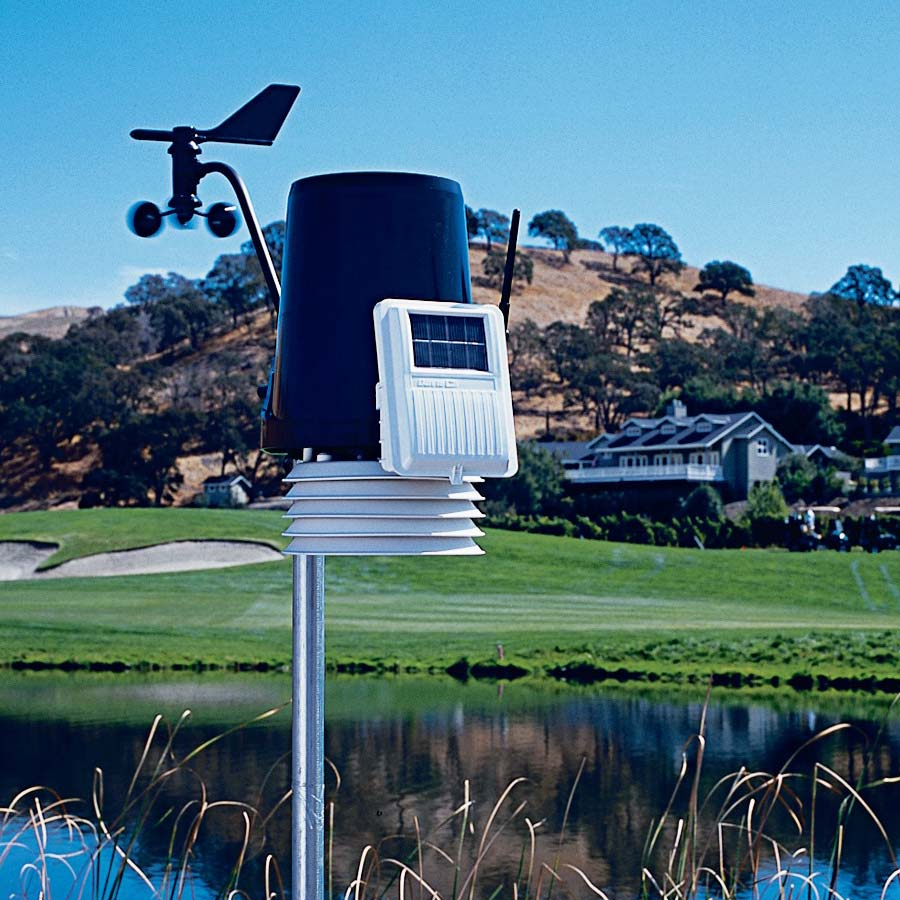
\includegraphics[height=4cm]{graphics/Davis_Vantage_Pro_2}}  
  \caption{Various price of portable weather stations}
  \label{fig:1}
\end{figure}

The goal of this project is to make an affordable, long-range communication
 data logger which result in more dens coverage in data logging and to assist scientific communities with limited budget. 